% Lab report template, 07/10/2016, v. 2. This template should be used in conjunction with the PDF file generated from it.

% This is the header of your report and will not feature in the report itself. It is useful to write things like the title of the document, the date and what version the document is here. The '%' symbol starts a comment line that will not appear in the final PDF.

% This document was written with TeXstudio and compiled with TeXworks, as TeXstudio cannot compile a pdf itself. Programs like TeXworks or MiKTeX can be used exclusively for writing and compiling a document, but are less user friendly than TeXstudio.

%This template is by no means a guide on how to use LaTeX to write documents, but a brief explanation of the major differences between Microsoft Word and LaTeX is given. LaTeX is an American program, and as such, some of the commands use the American way of spelling i.e. color instead of colour. 

%  USEFUL LINKS FOR LEARNING LaTeX:
%
%   http://en.wikibooks.org/wiki/LaTeX
%
%   http://www.andy-roberts.net/writing/latex/tables
%   http://www.andy-roberts.net/writing/latex/floats_figures_captions
%   http://www.andy-roberts.net/res/writing/latex/symbols.pdf
%

\documentclass[11pt]{article} %This sets the font size and the document class of your report. In this case we use 'article' as that is ideal for shorter reports. 

% LaTeX can be enhanced by the use of packages. These packages can do many things, a few of the most common and useful are used here. They are declared before the document proper, in what is known as the 'preamble'. Packages need to be installed when a .tex file compiles into a .pdf, but should do so automatically.

\usepackage[top=2.54cm, bottom=2.54cm, left=2.75cm, right=2.75cm]{geometry} %This sets the margins of the report.

\usepackage{tikz, float, pgfplots, xcolor, titlesec, amsmath, url, hanging, siunitx, graphicx, sectsty}

% Choose your citations style by commenting out one of the following groups. If you decide to change style, you should also delete the .bbl file that you will find in the same folder as your .tex and .pdf files.

% IEEE style citation:
\usepackage{cite}         % A package that creates references in the IEEE style. 
\newcommand{\citet}{\cite} % Use with cite only, so that it understands the natbib-specific \citet command
\bibliographystyle{ieeetr} % IEEE referencing (use in conjunction with the cite package)

%% Author-date style citation:
%\usepackage[round]{natbib} % A package that creates references in the author-date style, with round brackets
%\renewcommand{\cite}{\citep} % For use with natbib only: comment out for the cite package.
%\bibliographystyle{plainnat} % Author-date referencing (use in conjunction with the natbib package)


\usepackage{color} % Allows the colour of the font to be changed by using the '\color' command: This is just to support the blue comments in this template...use standard (black) text in your report.

\linespread{1.2} % Sets the spacing between lines of text.
\setlength{\parindent}{0cm}  % Suppresses indentation of text at the start of a paragraph

\begin{document} % This begins the document proper and ends the pre-amble

\begin{titlepage} % Begins the titlepage of the document
\begin{center} % Starts the beginning of an environment where all text is centered.

{\Huge The Chaotic Pendulum}\\[0.5cm] % [0.5cm] sets the distance between this line and the next.
\textit{Luna Greenberg} and \textit{Hamza Yasin}~\\[0.3cm] % The '\\' starts a new paragraph, and will only work after a paragraph has started, unless we use '~'.
\textit{11017146} and \textit{<Hamza put your student ID here>}~\\[0.3cm]
School of Physics and Astronomy~\\[0.3cm]
University of Manchester~\\[0.3cm]
Second year computational project report~\\[0.3cm]
April 2024~\\[2cm]


\end{center}
{\Large \textbf{Abstract}}~\\[0.3cm]
    <abstract>


\end{titlepage}
\pagenumbering{gobble} % This stops the title page being numbered
\clearpage
\pagenumbering{arabic} % sets the style of page numbering for the report
\setcounter{page}{2} % Starts the numbering at page 2 as typically the first page is not numbered

\newpage % Starts a new page to begin the report on.

\section{Introduction} 
% LaTeX automatically numbers sections and subsections when the command '\section{}' is used. This is useful in very long reports. It does not need a '\\' after it as LaTeX recognises it as a section header.
\label{intro}
% A label allows symbolic cross-referencing using the \ref{} command. 
% \label{} can appear in the text (when they refer to the preceding (sub)section title), equations, tables, or figures. 
% In this case, if you write "Section \ref{intro}" this will be rendered as "Section 1".


\section{Theory}
    Chaos can generally be seen through
    \begin{itemize}
        \item Sensitivity to initial conditions,
        \item Topological mixing, and
        \item Dense periodic orbits.
    \end{itemize}
    There are multiple maps and plots that can be made to examine these prperties. 
    The most common of these is the Poincar\'e section. This is a plot of the phase 
    space of the system, with position on the x-axis and velocity 
    on the y-axis. The Poincar\'e section is a useful tool for examining the periodic 
    orbits of the system, and the general method of using the state space of the system 
    is useful in analyzing the other two properties, topological mixing and initial condition
    sensitivity. Other tools include the bifurcation diagram, which shows the states of the
    system as a function of the driving force, as well as the Poincar\'e plot, which is a useful
    tool in examining the underlying structure of the system. \cite{Strogatz2000}\\

\section{Methodology}
    For simulating a system such as the chaotic pendulum, care must be taken to ensure the numerical methods 
    used are very precise, and to use a small enough time step to ensure that the system is accurately represented.
    Euler's method is simple and can be used to simulate the system, but it is not very accurate in contrast to
    the Runge-Kutta method, which uses half steps in the integration to give a better stepwise estimate. Although 
    more computationally expensive, the Runge-Kutta method is a good choice for this project, specifically
    RK4\cite{Strogatz2000}. RK4 was used to calculate the steps of angular velocity using the equation of
    motion for the forced, damped pendulum, and Euler's method was used to calculate the angle from the angular velocity, 
    as since the angular velocities are calculated discretely with RK4 there is no way to take the half step which is required 
    for another RK4 iteration in a way that would provide a benefit to the numerical computation. The equation of motion
    for this system\cite{PhysRevE.53.1579} is given by
    \begin{equation}
        \frac{d^2\theta}{dt^2} = -\frac{g}{R}\sin(\theta) - \frac{b}{M}\frac{d\theta}{dt} + F_d\sin(\Omega_d t)
    \end{equation}
    where $\theta$ is the angle of the pendulum, $t$ is the time since the initial condition, $g$ is the acceleration due to gravity,
    $R$ is the length of the pendulum, $b$ is the damping coefficient, $M$ is the mass of the pendulum, $F_d$ is the driving force,
    and $\Omega_d$ is the frequency of the driving force. This is a second order differential equation, requiring a mesh of 2d initial
    conditions. For this analysis, we assume $g=9.81\text{ms}^{-2}$, $R=10\text{m}$, $b=0.1\text{kgs}^{-1}$, and $M=10\text{kg}$ to all 
    be constant, and vary the driving force, $F_d$, and the frequency of the driving force, $\Omega_d$. The system will be analyzed using 
    Poincar\'e sections\cite{PoincareSection}, bifurcation diagrams \cite{Bifurcation}, Poincar\'e plots\cite{kamen1996poincare}, and the 
    Lyapunov exponent\cite{Lyapunov}, as well as a qualitative analysis of the phase space evolution of the system.\\
    \subsection{Poincar\'e Sections}
        Poincar\'e sections for this project were constructed by analyzing individual initial conditions and plotting the position
        of the pendulum against the velocity of the pendulum until the system reached a periodic orbit.  Determining what makes
        a periodic orbit in a chaotic system with numerical methods is not completely obvious - the error in the numerical method
        was tracked for each initial condition, and the periodic orbit was determined to be when the point returned to within the
        error of the initial condition. The error was determined by the step size of the Runge-Kutta method and Euler method and then
        propagated forward through the equation of motion.\\\vspace{3mm}

        The Poincar\'e section will look different depending on whether or not the system is chaotic. If the system is not chaotic,
        which is theoretically what should be recovered in the case of a small driving force, the Poincar\'e section will look like
        an ellipse or a circle. If the system is chaotic, the Poincar\'e section will look like a dense cloud of points, visually
        not appearing to have any structure. We can use qualitative analysis of the structure of the graph and whether or not such
        graphs are calculable in the given time frame to determine the chaotic behavior of the system, since a chaotic system should
        have dense periodic orbits that don't closely resemble ellipses.\\
    \subsection{Bifurcation Diagrams}
        Bifurcation diagrams were constructed by analyzing the system of the pendulum as a function of the driving force. The system
        was simulated for a range of driving forces, and the system of the pendulum was plotted for many initial conditions over a 
        long time frame. The bifurcation diagram was then analyzed for periodic orbits and chaotic behavior. Bifurcation diagrams were
        created for both the angle of the system and the angular velocity, and were made using a 2d histogram on a log scale of counts\\\vspace{3mm}

        A spread bifurcation diagram is indicative of a chaotic system, while a rigid bifurcation diagram is indicative of a non-chaotic
        system. The system may become chaotic at a certain driving force, and the bifurcation diagram can be used to determine the
        driving force at which it does.\\
    \subsection{Poincar\'e Plots}
        Poincar\'e plots were constructed by plotting the position of the pendulum at a given point on the x axis and the next position of
        the pendulum on the y axis to get a sense of the underlying structure of the system. Structure in the Poincare plot can be indicative
        of certain patterns of behavior and are often used to determine the governing structure of the system, though the Poincar\'e plot
        is not as useful for determining the chaotic behavior of the system as other methods, and would require more in-depth analysis to reach
        conclusions of chaos.\\
    \subsection{Lyapunov Exponent}
        The Lyapunov exponent is a measure of the sensitivity to initial conditions of a system. It measures the rate at which
        adjacent points in the phase space diverge from each other. The Lyapunov exponent applies locally to two adjacent points in phase
        space, but may not reflect the overall behavior for the system for cases such as this one where the system is modular. It may therefore
        be more useful to analyze the difference graphs from which the Lyapunov exponent would be constructed.
    \subsection{Phase Space Analysis}
        The phase space is a 2d plot of the angle of the pendulum on the x-axis and the angular velocity of the pendulum on the y-axis. 
        The phase space is a useful tool for analyzing the behavior of the system, and can be used qualitatively to assess sensitivity 
        to initial conditions and topological mixing. A full GUI was created for analyzing the system qualitatively, however the format
        of the lab report means that only certain snapshots can be shown, and a link to mp4 animations will be provided, as well as a link
        to the project on GitHub, which can be run with python to show the GUI.\\
\section{Results}
    \subsection{Poincar\'e Sections}
    The forces and frequencies analyzed for the Poincar\'e sections were chosen qualitatively based on the bifurcation diagrams. Below are
    three groups of Poincar\'e sections for driving forces of 0.5, 1.0, and 2.0 Newtons, organized into columns of uniform driving frequency. 
    \begin{figure}[H]
        \centering
        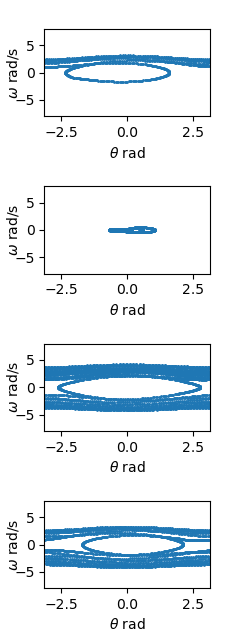
\includegraphics[width=0.15\textwidth]{pcr_0.5_0.15.png}
        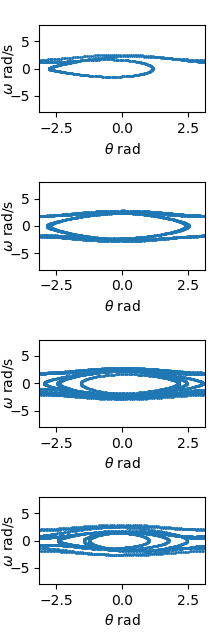
\includegraphics[width=0.15\textwidth]{pcr_0.5_0.3.png}
        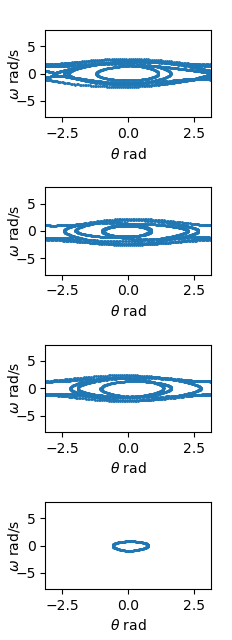
\includegraphics[width=0.15\textwidth]{pcr_0.5_0.5.png}
        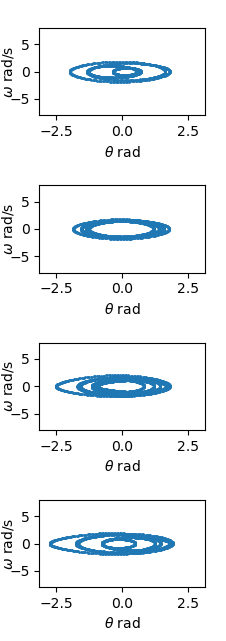
\includegraphics[width=0.15\textwidth]{pcr_0.5_1.0.png}
        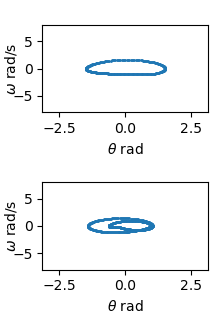
\includegraphics[width=0.15\textwidth]{pcr_0.5_1.5.png}
        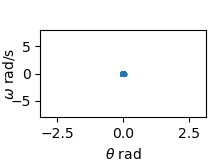
\includegraphics[width=0.15\textwidth]{pcr_0.5_3.0.png}
        \caption{Poincar\'e sections of the chaotic pendulum for a driving force of a half Newton, as a function of the driving frequency $\Omega_d$=0.15, 0.3, 0.5, 1.0, 1.5, and 3.0 (from left to right).}
    \end{figure}
    \begin{figure}[H]
        \centering
        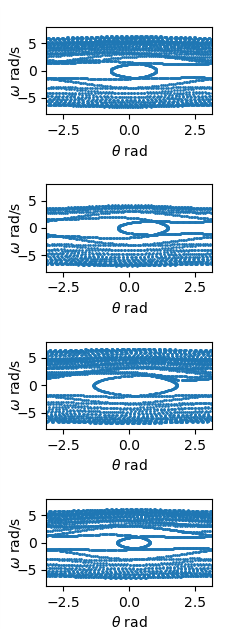
\includegraphics[width=0.15\textwidth]{pcr_1.0_0.15.png}
        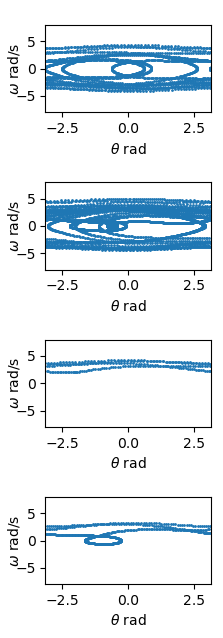
\includegraphics[width=0.15\textwidth]{pcr_1.0_0.3.png}
        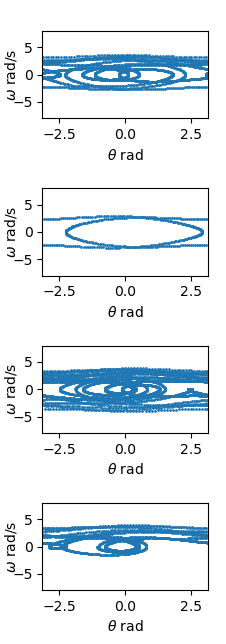
\includegraphics[width=0.15\textwidth]{pcr_1.0_0.5.png}
        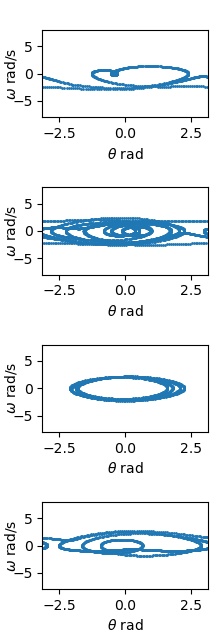
\includegraphics[width=0.15\textwidth]{pcr_1.0_1.0.png}
        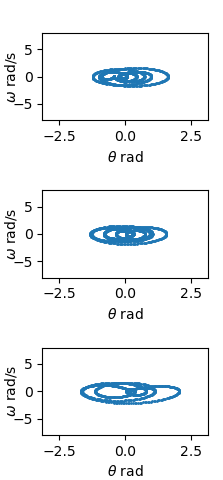
\includegraphics[width=0.15\textwidth]{pcr_1.0_1.5.png}
        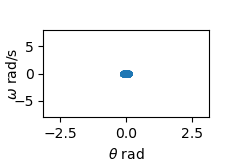
\includegraphics[width=0.15\textwidth]{pcr_1.0_3.0.png}
        \caption{Poincar\'e sections of the chaotic pendulum for a driving force of one Newton, as a function of the driving frequency $\Omega_d$=0.15, 0.3, 0.5, 1.0, 1.5, and 3.0 (from left to right).}
    \end{figure}
    \begin{figure}[H]
        \centering
        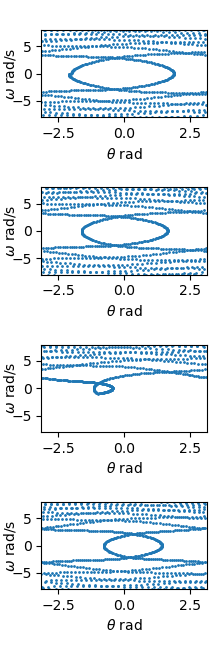
\includegraphics[width=0.15\textwidth]{pcr_2.0_0.15.png}
        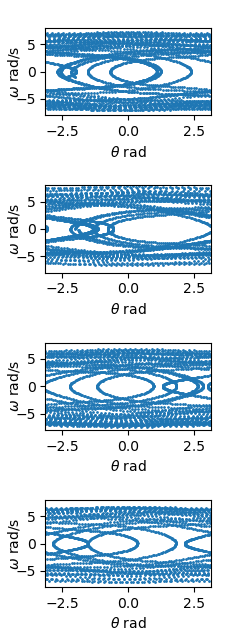
\includegraphics[width=0.15\textwidth]{pcr_2.0_0.3.png}
        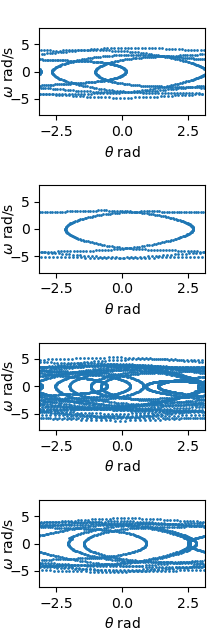
\includegraphics[width=0.15\textwidth]{pcr_2.0_0.5.png}
        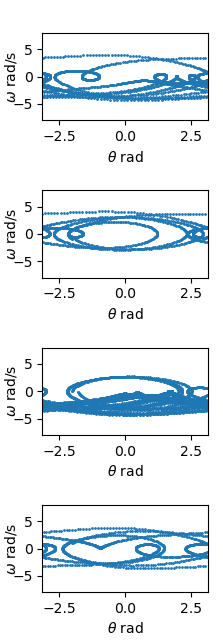
\includegraphics[width=0.15\textwidth]{pcr_2.0_1.0.png}
        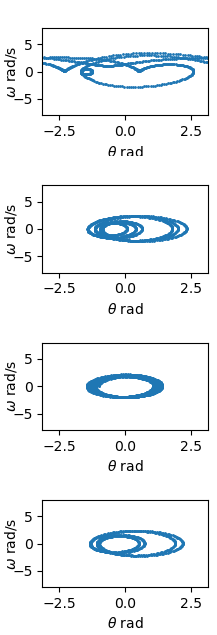
\includegraphics[width=0.15\textwidth]{pcr_2.0_1.5.png}
        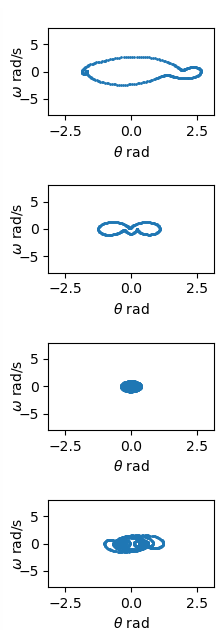
\includegraphics[width=0.15\textwidth]{pcr_2.0_3.0.png}
        \caption{Poincar\'e sections of the chaotic pendulum for a driving force of two Newtons, as a function of the driving frequency $\Omega_d$=0.15, 0.3, 0.5, 1.0, 1.5, and 3.0 (from left to right).}
        \label{fig:poincare}
    \end{figure}
    Two main qualitative observations can be made from the Poincar\'e sections - the first is that at higher values of the driving frequencies,
    the iterator has a harder time finding 4 periodic orbits, indicating that the periodic orbits are less dense at those values, and thus
    the system is less chaotic. The second qualitative observation is that the system is more chaotic at higher driving forces, as can be seen by the
    density of the points and lack of ellipse structure in the Poincar\'e sections for higher forces that is well observed at lower force values. These
    qualitative differences help demonstrate the chaotic behavior of the system at higher force and lower frequency values.\\
    \subsection{Bifurcation Diagrams}
    Below are a selection of bifurcation diagrams from the dynamic program that was created to analyze the chaotic pendulum. Due to the
    amount of data points involved and the limitations of scatter plots on performance, a log-scaled 2d histogram was used to represent the
    data. The values of the driving frequency were chosen based on qualitative analysis of the system.
    \begin{figure}[H]
        \centering
        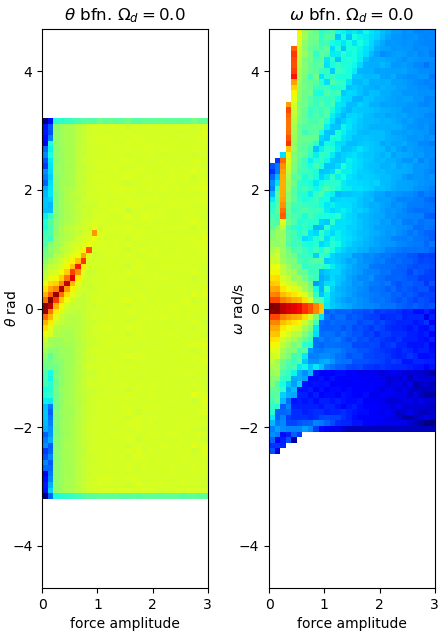
\includegraphics[width=0.2\textwidth]{bfn_0.0.png}
        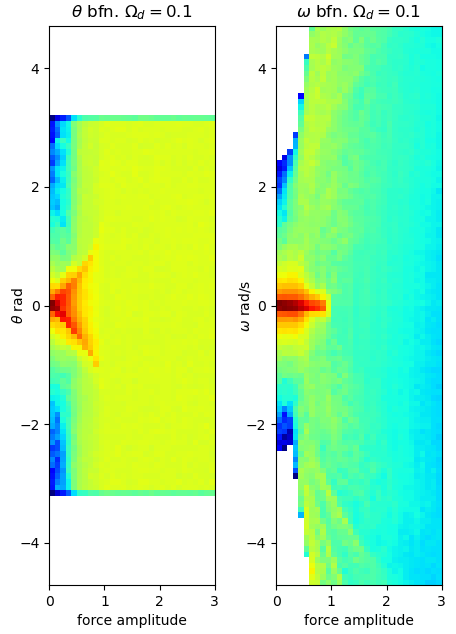
\includegraphics[width=0.2\textwidth]{bfn_0.15.png}
        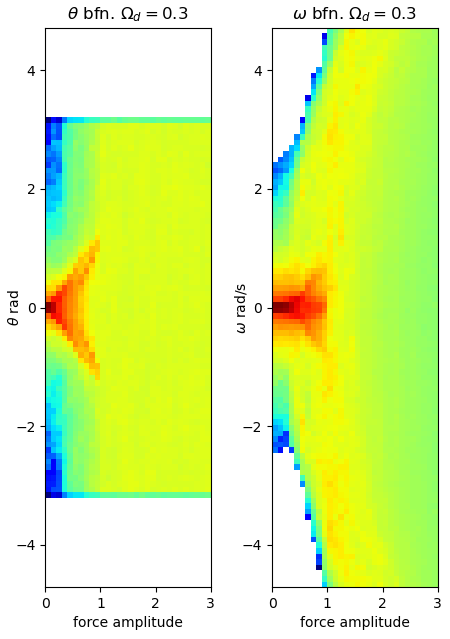
\includegraphics[width=0.2\textwidth]{bfn_0.3.png}
        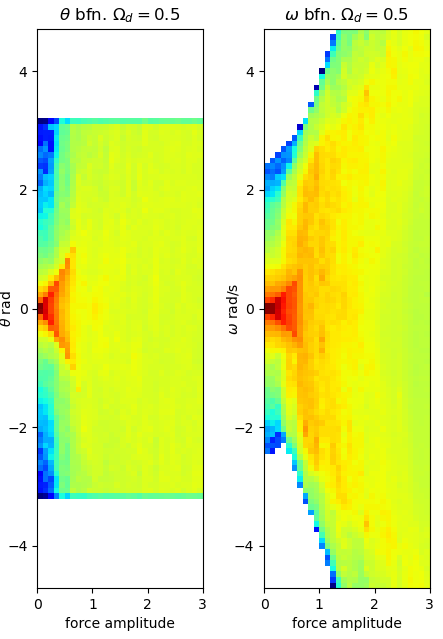
\includegraphics[width=0.2\textwidth]{bfn_0.5.png}
        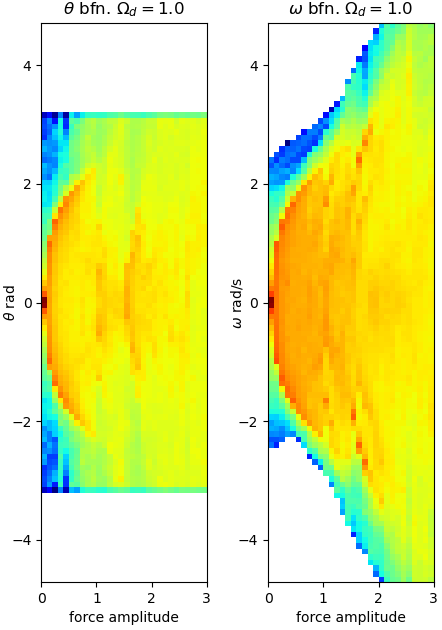
\includegraphics[width=0.2\textwidth]{bfn_1.0.png}
        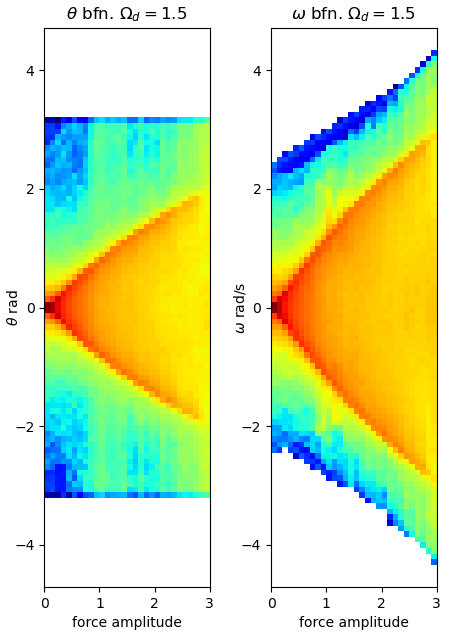
\includegraphics[width=0.2\textwidth]{bfn_1.5.png}
        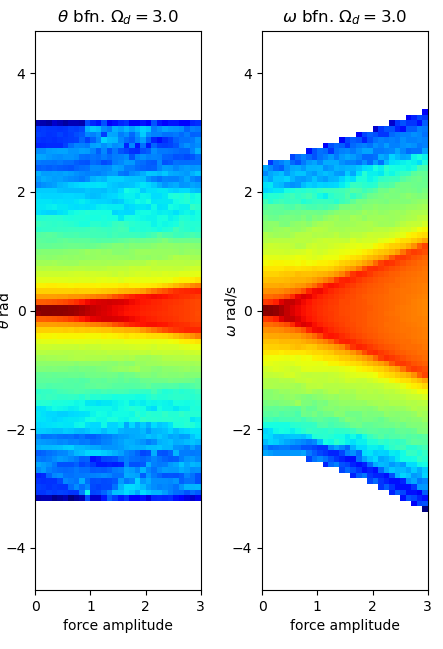
\includegraphics[width=0.2\textwidth]{bfn_3.0.png}
        \caption{Bifurcation diagrams of the angle and angular velocity of the pendulum as a function of the driving force}
        \label{fig:bifurcation}
    \end{figure}
    Using these bifurcation diagrams, we observed the system to generally be highly chaotic above a driving force of one Newton, and to generally
    be moderately to lightly chaotic below a driving force of one Newton, becoming non-chaotic closer to zero. This result was used to inform
    the selection of driving forces for the Poincar\'e sections. The chaos of the system can be seen through the bifurcation diagrams based on their
    spread, and as can be seen in every case the diagram becomes more spread for higher force values, with the most rapid spreading for values of the
    driving frequency between $0.15$ and $1.5$ Hz. Below this range the frequency is so low that the force becomes either dominant in the motion of the
    pendulums or negligible depending on its magnitude, and above the range the force is acting too quickly for many chaotic effects to occur, and a
    dense collection of points can be seen at a smaller spread of angles and angular velocities.\\
    \subsection{Poincar\'e Plots}
    Poincar\'e plots were established for forces and frequencies of interest. They were constructed as scatter plots to get an idea of the spread
    of the data without diving too deep into the distribution of the data.
    \begin{figure}[H]
        \centering
        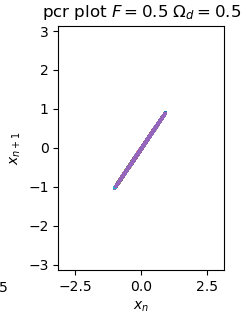
\includegraphics[width=0.3\textwidth]{pcp_0.5_0.5.png}
        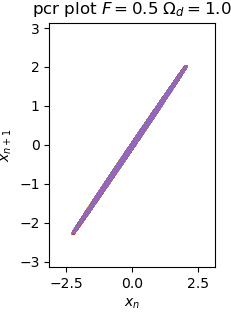
\includegraphics[width=0.3\textwidth]{pcp_0.5_1.0.png}
        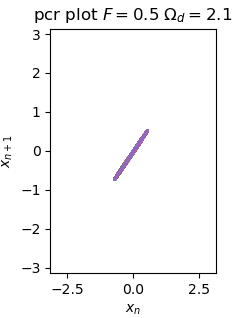
\includegraphics[width=0.3\textwidth]{pcp_0.5_2.0.png}
        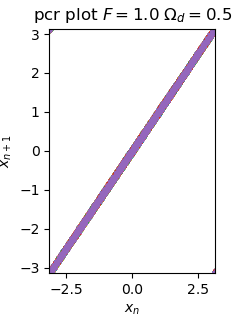
\includegraphics[width=0.3\textwidth]{pcp_1.0_0.5.png}
        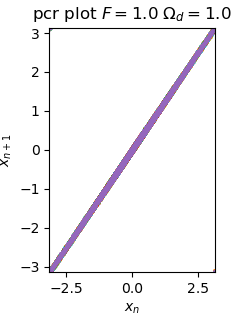
\includegraphics[width=0.3\textwidth]{pcp_1.0_1.0.png}
        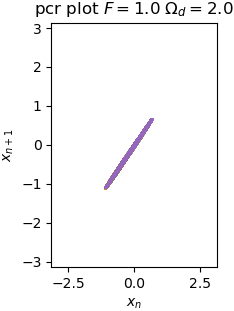
\includegraphics[width=0.3\textwidth]{pcp_1.0_2.0.png}
        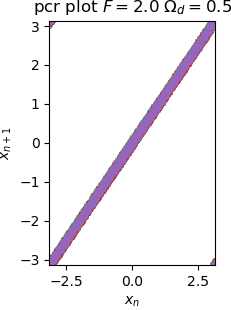
\includegraphics[width=0.3\textwidth]{pcp_2.0_0.5.png}
        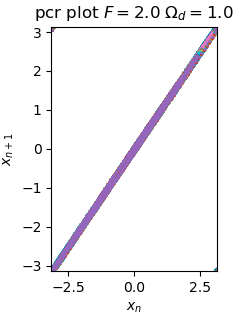
\includegraphics[width=0.3\textwidth]{pcp_2.0_1.0.png}
        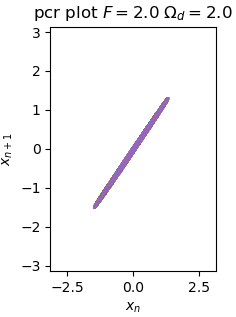
\includegraphics[width=0.3\textwidth]{pcp_2.0_2.0.png}
        \caption{Poincar\'e plots of the chaotic pendulum for different driving forces and driving frequencies.}
    \end{figure}
    It can be seen that the Poincar\'e plots are the most spread for higher values of the force and lower values of the frequency, which can be
    an indicator of chaotic behavior. What's most interesting about the Poincar\'e plots is that they all follow a similar structure, a line of
    some width from the bottom left to the top right of the graph. This tells us that for each angle, the system will either move to the left or
    to the right with some relatively predictable velocity. These graphs aren't very useful for determining the chaotic behavior of the system,
    but they are useful for determining the underlying structure of the system, and showing that chaos does not necessarily mean that the system
    is unpredictable.\\
    \subsection{Lyapunov Exponent}
    While the Lyapunov Exponent could be calculated numerically, we thought it more appropriate to use a qualitative analysis of the system and
    the difference data to assess whether or not the system was chaotic and its sensitivity to initial conditions. The reason for this is that
    the graph that would be used to determine the Lyapunov exponent contains far more information about the behavior of different initial conditions
    and about the growth or decay of the differences than a single number would. Due to space concerns on the GUI the force and frequency were not
    included in the titles of the graphs, but they follow the same layout with the same values as the Poincar\'e plots
    \begin{figure}[H]
        \centering
        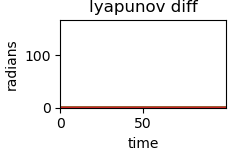
\includegraphics[width=0.3\textwidth]{lya_0.5_0.5.png}
        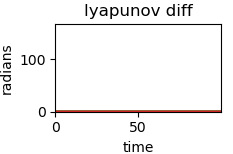
\includegraphics[width=0.3\textwidth]{lya_0.5_1.0.png}
        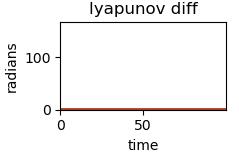
\includegraphics[width=0.3\textwidth]{lya_0.5_2.0.png}
        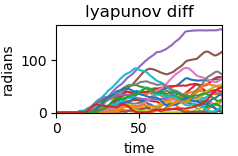
\includegraphics[width=0.3\textwidth]{lya_1.0_0.5.png}
        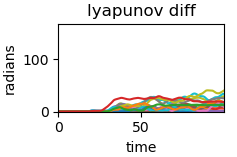
\includegraphics[width=0.3\textwidth]{lya_1.0_1.0.png}
        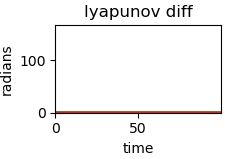
\includegraphics[width=0.3\textwidth]{lya_1.0_2.0.png}
        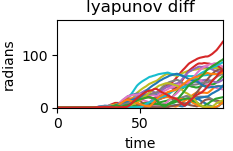
\includegraphics[width=0.3\textwidth]{lya_2.0_0.5.png}
        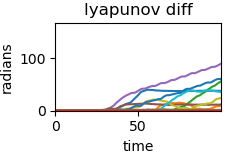
\includegraphics[width=0.3\textwidth]{lya_2.0_1.0.png}
        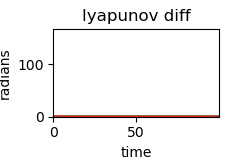
\includegraphics[width=0.3\textwidth]{lya_2.0_2.0.png}
        \caption{Poincar\'e plots of the chaotic pendulum for different driving forces and driving frequencies.}
    \end{figure}
    The Lyapunov exponent graphs are a much better qualitative indicator of chaos than the Poincar\'e plots for the same force and frequency
    magnitudes. The graphs that aren't all within one rotation ($2\pi$) of each other show an extreme sensitivity to initial conditions, which
    tends to happen for the lower frequency and higher force values. The graphs themselves aren't particularly exponential over large scales, which
    becomes even more relevant when you consider that these are the un-modded difference graphs - if you were to observe the experiment physically
    where $2\pi = 0$, it becomes impossible to see an exponential difference in initial conditions. The choice to use qualitative analysis with regard
    to the Lyapunov exponent becomes apparent - the point at which local exponential differences become outdone by global patterns is arbitrary, and
    quantitative analysis would have little use.\\

    \subsection{Phase Space Analysis}
\section{Conclusions}

\bibliography{report_template_library} % Specifies the bibliography file where our references are stored. If the library file and document are not in the same folder then the file path must also be included.


\end{document}
